\documentclass[11pt,a4paper]{article}

\usepackage[top=1.2in,bottom=1.1in,left=1in,right=1in,headheight=14pt,headsep=20pt]{geometry}
\usepackage[T1]{fontenc}
\usepackage[utf8]{inputenc}
\usepackage{mathptmx}
\usepackage{microtype}
\usepackage{graphicx}
\usepackage{booktabs}
\usepackage{amsmath}
\usepackage{amssymb}
\usepackage{caption}
\usepackage{enumitem}
\usepackage{xcolor}
\usepackage{float}
\usepackage{tikz}
\usepackage{fancyhdr}
\usepackage{sectsty}
\definecolor{hitnavy}{HTML}{0D1B6E}
\definecolor{hitblue}{HTML}{134989}
\definecolor{hitteal}{HTML}{1FA6C1}
\definecolor{hittealdk}{HTML}{16828E}
\usepackage[authoryear,round]{natbib}
\usepackage[hidelinks]{hyperref}

\captionsetup{font=small,labelfont=bf}
\setlist{nosep,leftmargin=1.4em}
\graphicspath{{./}{../visuals/}}

\sectionfont{\color{hitnavy}\large\bfseries}
\subsectionfont{\color{hittealdk}\bfseries}
\pagestyle{fancy}
\fancyhf{}
\renewcommand{\headrulewidth}{0pt}
\renewcommand{\footrulewidth}{0pt}
\fancyhead[C]{\begin{tikzpicture}[remember picture,overlay]
  \shade[left color=hitblue,right color=hitteal] ([yshift=-1.25cm]current page.north west) rectangle (current page.north east);
  \node[anchor=north west,fill=white,rounded corners=2pt,inner sep=2.5pt] at ([xshift=1.5cm,yshift=-0.16cm]current page.north west) {
\includegraphics[height=0.6cm]{hit_logo.png}};
  \node[anchor=north east,text=white,align=right] at ([xshift=-1.5cm,yshift=-0.3cm]current page.north east) {\footnotesize\bfseries Faculty of Digital Medical Technologies\\[1pt]\scriptsize LLM / Generative AI $\cdot$ Spring 2026};
\end{tikzpicture}}
\fancyfoot[C]{\begin{tikzpicture}[remember picture,overlay]
  \shade[left color=hitblue,right color=hitteal] (current page.south west) rectangle ([yshift=0.85cm]current page.south east);
  \node[anchor=west,text=white] at ([xshift=1.5cm,yshift=0.42cm]current page.south west) {\scriptsize K.T.};
  \node[text=white] at ([yshift=0.42cm]current page.south) {\scriptsize\bfseries \thepage};
  \node[anchor=east,text=white] at ([xshift=-1.5cm,yshift=0.42cm]current page.south east) {\scriptsize HIT \textemdash\ Holon Institute of Technology};
\end{tikzpicture}}

\title{\vspace{-1.5em}\textbf{Dominant Psychosocial Response and Distress\\
Classification in Oncology-Related Messages:\\[2pt]
\large A Synthetic, Label-Leakage-Controlled NLP Study}}
\author{K.T.\\
\small Holon Institute of Technology (HIT)\\
\small LLM / Generative AI course --- A.A.}
\date{}

\begin{document}
\thispagestyle{fancy}
\begin{center}
{
\includegraphics[width=5.2cm]{hit_logo.png}}\\[8pt]
{\color{hitteal}\rule{3.8cm}{1.4pt}}\\[12pt]
{\Large\bfseries\color{hitnavy}Dominant Psychosocial Response and Distress\\[2pt]Classification in Oncology-Related Messages}\\[5pt]
{\large\color{hittealdk}A Synthetic, Label-Leakage-Controlled NLP Study}\\[10pt]
{\normalsize K.T.}\\[2pt]
{\small Holon Institute of Technology (HIT) \textemdash\ Faculty of Digital Medical Technologies}\\[1pt]
{\small LLM / Generative AI course \textemdash\ A.A.}
\end{center}
\vspace{6pt}

\begin{abstract}
\noindent
We study two-label classification of oncology-related messages: the dominant \emph{psychosocial
response} (seven classes: anxiety, sadness, anger, hope, guilt, denial, acceptance) and the
\emph{intensity of distress} (three ordinal levels: low, medium, high). We found no public corpus
with this exact joint seven-response and three-level distress framing, and emotional labels are
subjective and costly to annotate; we therefore construct a
fully synthetic corpus using attribute-based generation under a strict \emph{label-leakage ban} (the
generated text never explicitly names the target response label), and we audit every item with two independent
large-language-model judges, organizing the corpus into strict, silver, and consensus quality tiers. We generated 2,033 candidate
messages, obtained 2,025 valid audited messages, and retained 1,273 model-ready items across these
tiers. We compare three model families on both tasks --- a sparse lexical
baseline (TF-IDF with logistic regression), a fine-tuned transformer (DistilBERT), and an
off-the-shelf zero-shot model (BART-MNLI) --- using macro-F1, ordinal-aware metrics, and a
5000-resample paired bootstrap, and we validate the synthetic labels against a blind human annotator
on a 67-item test set. On response classification a lexical model has the highest point estimate (macro-F1 0.856), while its
difference from the best transformer is not statistically resolved; on distress the transformer leads on the mean (0.864) but its advantage
over the lexical model is not statistically resolved on 67 items, whereas both supervised systems
reliably outperform zero-shot. We further find that more synthetic data is not uniformly better, and
that residual errors concentrate at the low/medium distress boundary rather than at severe failures.
\end{abstract}

\section{Introduction}
A cancer diagnosis carries a heavy psychosocial burden for patients and caregivers, and supportive-care
teams increasingly seek to triage the emotional state behind patient-generated text such as forum
posts, messages, and intake notes. Two questions are clinically relevant: \emph{which psychosocial
response dominates} a message, and \emph{how intense the distress} is. Automating this at scale is
attractive, but two obstacles stand in the way. First, there is no public labeled dataset for this
exact joint framing. Second, emotional labels are subjective and expensive to obtain, and a naive
classifier can ``cheat'' on explicit emotion keywords rather than learning the underlying state.

This project addresses both obstacles by generating its own data and by studying which modelling
approach is actually justified for the task. Our contributions are:
\begin{itemize}
  \item a novel two-label task on oncology messages (seven-class psychosocial response and a
        three-level ordinal distress label), distinct from broad sentiment classification;
  \item a fully synthetic, attribute-controlled corpus built under a strict label-leakage ban and
        audited by two independent LLM judges into strict/silver/consensus quality tiers;
  \item a controlled comparison of three model families on both tasks, with significance testing via
        a 5000-resample paired bootstrap and an independent blind human validation; and
  \item an analysis of how the amount of synthetic data affects each model, plus a consolidated error
        analysis identifying where the remaining errors lie.
\end{itemize}

Figure~\ref{fig:overview} summarizes the pipeline and the headline results.

\begin{figure}[t]
  \centering
  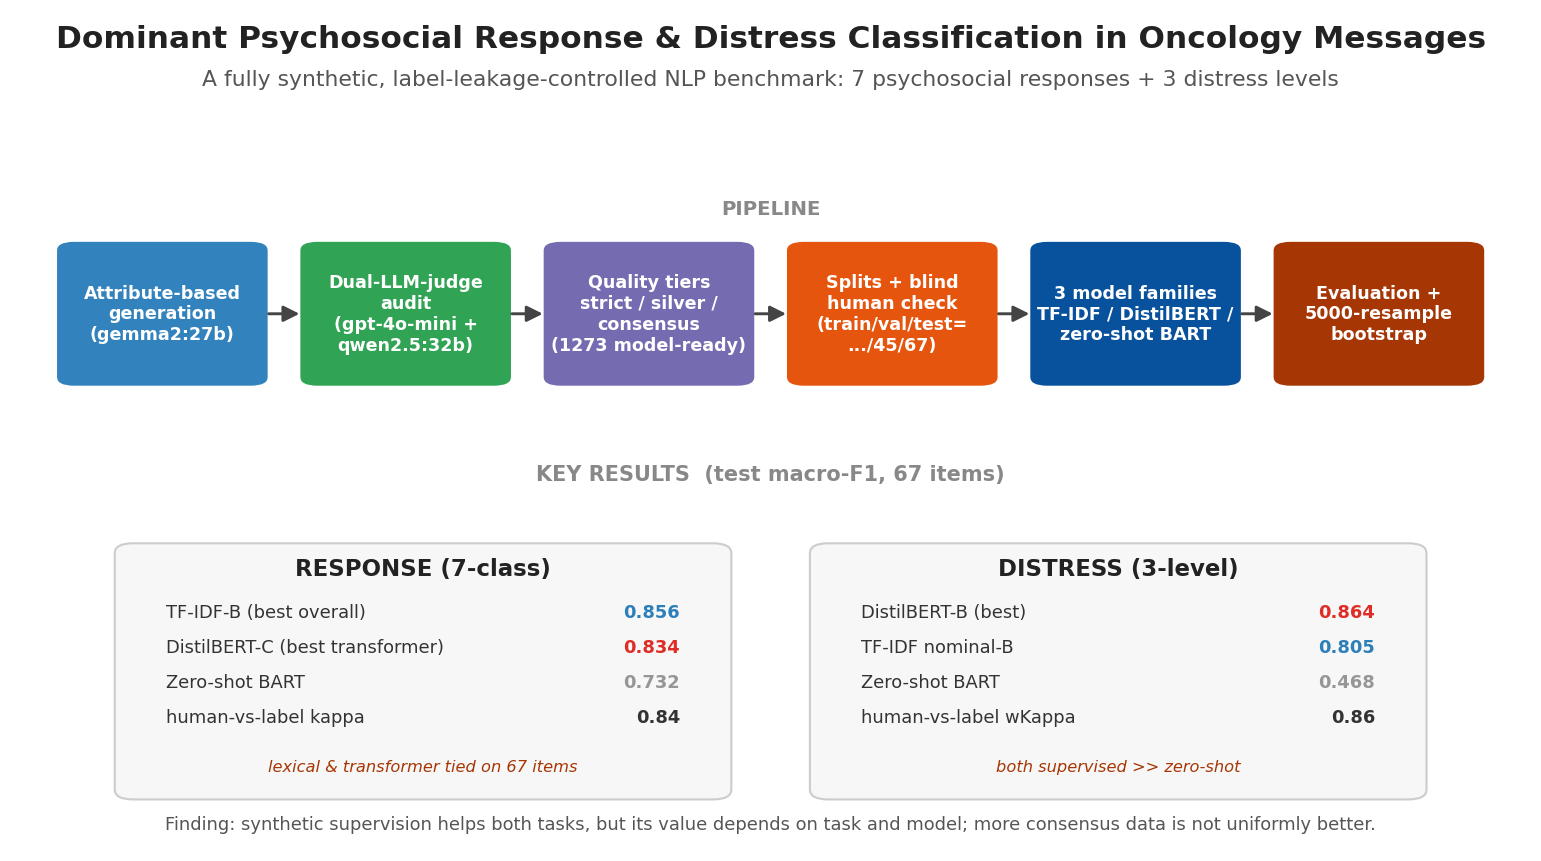
\includegraphics[width=0.98\linewidth]{visual_abstract.png}
  \caption{Overview of the pipeline (attribute-based generation, dual-LLM-judge audit, quality tiers,
  splits with a blind human check, three model families, and bootstrap evaluation) and the headline
  test results for both tasks.}
  \label{fig:overview}
\end{figure}

\section{Related Work}
Our method draws on three lines of recent work and is most directly comparable to one domain study.
\citet{yu2023} introduce attribute-conditioned synthetic data generation, in which a language model is
prompted with sampled attributes to control diversity; they show that attribute diversity improves
downstream utility but that generation can introduce systematic bias --- exactly the trade-off we
manage when sampling oncology attributes. \citet{li2023} study when LLM-generated synthetic data helps
text classification and report that synthetic data becomes \emph{less effective as task subjectivity
rises}; because emotional labels are highly subjective, this motivates our strict auditing, quality
tiers, and human check. \citet{zheng2023} formalize the LLM-as-judge paradigm, showing that strong LLM
judges reach over 80\% agreement with human experts while exhibiting position, verbosity, and
self-enhancement biases; this provides a methodological precedent for scalable LLM-based evaluation and
documents the biases that motivate our use of two independent judges and a human validation. Finally,
\citet{xu2026} classify emotional tone in online cancer peer-support posts using LLM-based annotation
and a range of models (TF-IDF logistic regression, random forest, LightGBM, GRU, and a fine-tuned
ALBERT) over three tone classes; this is the closest domain baseline. Our task differs in that we
predict seven fine-grained psychosocial responses (rather than negative/neutral/positive), add a
separate ordinal distress task, use a fully synthetic attribute-controlled corpus with dual-judge
auditing and quality tiers, and explicitly analyze human ambiguity and the divergence between the
synthetic annotation policy and human interpretation. A broad survey of NLP for mental-illness
detection \citep{zhang2022} situates the wider domain.

Finally, this project continues a line of work at the host institution on constructing controlled
synthetic benchmarks for evaluating language models on text classification. \citet{apartsin2025str}
build a synthetic benchmark through controlled paraphrasing and deliberate information removal and
compare discriminative and generative models for classifying semantic relations between text pairs,
releasing both the dataset and its generation code; our attribute-controlled corpus and three-family
model comparison apply the same methodology to psychosocial response and distress. In the clinical
domain, \citet{werthaim2026} generate synthetic patient cases and simulate interactions with GPT-4.1
and GPT-4o-mini agents to benchmark diagnostic questioning, and \citet{mama2025} benchmark language
models on noisy patient narratives; these motivate, respectively, our use of an LLM judge
(\texttt{gpt-4o-mini}) over synthetic medical text and our explicit modelling of message noise.

\section{Task and Data}

\subsection{Task definition}
Given a single English oncology-related message, we predict two labels with separate models:
$f(\text{text}) \rightarrow (\text{response} \in \mathcal{R},\ \text{distress} \in \{\text{low},
\text{medium}, \text{high}\})$, where $\mathcal{R} = \{$anxiety, sadness, anger, hope, guilt, denial,
acceptance$\}$. Distress is ordinal: the error low$\rightarrow$high is treated as worse than
low$\rightarrow$medium, so distress is evaluated with ordinal-aware metrics.

\subsection{Attribute-based synthetic generation}
The corpus is fully synthetic (no real patient data). Each message is generated from a sampled
combination of attributes --- role (patient/caregiver/\ldots), cancer stage, cancer type, tone,
channel, age group, length, and a noise flag --- so that the attribute grid enforces diversity and
coverage. A local generator (\texttt{gemma2:27b} via Ollama) is conditioned on the sampled attributes
\emph{and} an intended (response, distress) label and asked to write a natural message that expresses
that state \emph{without ever explicitly naming the target response label}. This label-leakage ban reduces the risk that a classifier
succeeds by detecting explicit class-name tokens. Malformed outputs and explicit constraint violations were rejected.
Label drift was audited separately: items were either rejected or retained with consensus labels when
both judges confidently agreed on an alternative interpretation.

\subsection{Dual-LLM-judge auditing and quality tiers}
Two independent judges (\texttt{gpt-4o-mini} and \texttt{qwen2.5:32b}) read each message \emph{without}
seeing the intended label and predict the two labels. Each item is assigned to a quality tier. Strict
items matched both intended labels according to both judges with confidence at least 4 and no
ambiguity. Silver items also matched both intended labels according to both judges, but had confidence
at least 3 rather than meeting the strict threshold. Consensus items were those for which both judges
confidently agreed with each other on labels that differed from the intended labels; their final
labels were set to the judge consensus. The union of these three tiers forms the model-ready corpus
(Table~\ref{tab:data}).

\subsection{Splits and human validation set}
We build a frozen test set of 67 strict-tier items and a validation set of 45 items (seed 42), with
three nested training tiers: \emph{train\_A} (strict only, 359), \emph{train\_B} (strict$+$silver, 434),
and \emph{train\_C} (strict$+$silver$+$consensus, 1161). The three tiers let us measure whether more
synthetic data of decreasing purity helps. The 67-item test set was independently re-annotated by a
human (Section~\ref{sec:human}) to validate the synthetic labels before any model was trusted.

\begin{table}[t]
  \centering
  \small
  \caption{Corpus construction funnel and the data splits (seed 42). Only the model-ready subset was
  used in the supervised experiments.}
  \label{tab:data}
  \begin{tabular}{@{}lr@{\hspace{2.4em}}lr@{}}
    \toprule
    \multicolumn{2}{c}{\textbf{Corpus construction}} & \multicolumn{2}{c}{\textbf{Data splits}}\\
    \cmidrule(r){1-2}\cmidrule(l){3-4}
    Stage & Count & Split & Size\\
    \midrule
    candidate messages       & 2033 & test                 & 67\\
    valid audited            & 2025 & validation           & 45\\
    \quad model-ready (used) & \textbf{1273} & train\_A (strict)    & 359\\
    \quad\quad strict        & 471  & train\_B (+silver)   & 434\\
    \quad\quad silver        & 75   & train\_C (+consensus) & 1161\\
    \quad\quad consensus     & 727  & & \\
    \quad review-only        & 752  & & \\
    needs-rejudging          & 8    & & \\
    \bottomrule
  \end{tabular}
\end{table}

\subsection{Exploratory data analysis}
The model-ready corpus ($n=1273$) is class-imbalanced. For response, the class counts are anxiety 458,
guilt 234, hope 201, sadness 177, anger 90, denial 57, and acceptance 56; for distress they are low 333,
medium 694, and high 246. Messages are short (median 31 words; range 4--107). Figure~\ref{fig:eda}
summarizes the distributions. We stress that these distributions reflect the generation and auditing
pipeline and are \emph{not} estimates of real-world prevalence.

\begin{figure}[t]
  \centering
  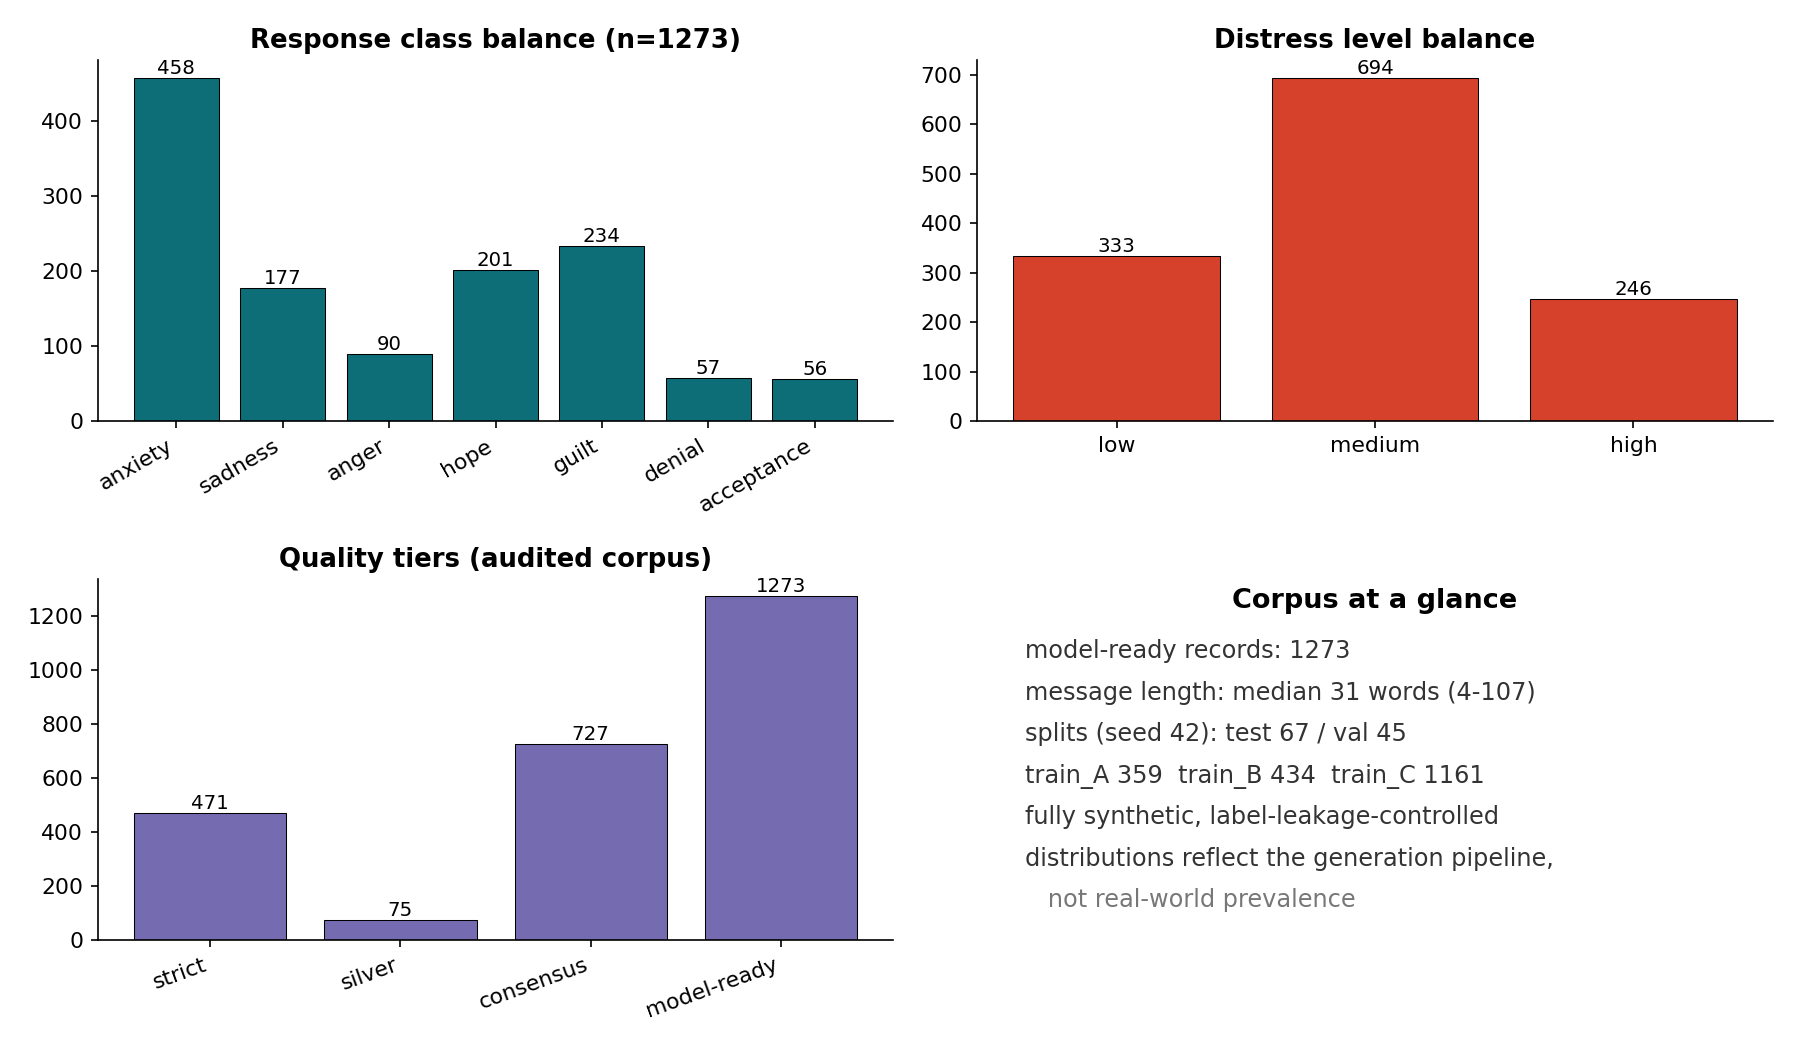
\includegraphics[width=0.92\linewidth]{eda_overview_slide.png}
  \caption{Exploratory data analysis of the model-ready corpus: response and distress class balance,
  quality-tier sizes, and summary statistics.}
  \label{fig:eda}
\end{figure}

\section{Methods}

\subsection{Models}
We compare three model families on both tasks, alongside a trivial floor:
\begin{itemize}
  \item \textbf{Majority class}: predicts the most frequent label (sanity floor).
  \item \textbf{TF-IDF $+$ logistic regression}: class-weighted multinomial logistic regression on
        TF-IDF features. For distress we evaluate two variants: a \emph{nominal} three-class model and
        an \emph{ordinal} two-threshold formulation ($P(y>\text{low})$, $P(y>\text{medium})$) with
        validation-tuned thresholds and a monotonic correction.
  \item \textbf{DistilBERT} (\texttt{distilbert-base-uncased}): a fine-tuned transformer with a
        classification head, trained separately for each task with class-weighted cross-entropy.
  \item \textbf{Zero-shot BART-MNLI} (\texttt{facebook/bart-large-mnli}): off-the-shelf
        natural-language-inference zero-shot classification (two prompt templates averaged for
        distress).
\end{itemize}

\subsection{Training and hyperparameters}
DistilBERT is fine-tuned with the regime in Table~\ref{tab:hyper}, identical for both tasks. A separate
model is trained for each tier (A/B/C), and all transformer results are reported as the mean and
standard deviation over five random seeds.

\begin{table}[H]
  \centering
  \small
  \caption{DistilBERT fine-tuning configuration (identical for both tasks).}
  \label{tab:hyper}
  \begin{tabular}{@{}ll@{}}
    \toprule
    Setting & Value\\
    \midrule
    Base model & \texttt{distilbert-base-uncased}\\
    Seeds & 13, 42, 73, 101, 2026 (mean $\pm$ std)\\
    Max epochs & 12, early stop (patience 2, $\Delta=0.005$ val macro-F1)\\
    Batch size & 16\\
    Learning rate & $2\times10^{-5}$ (linear schedule, warmup 0.10)\\
    Weight decay / grad clip & 0.01 / 1.0\\
    Max token length & 128\\
    Loss & class-weighted cross-entropy (weight cap 5.0)\\
    Model selection & best validation macro-F1\\
    \bottomrule
  \end{tabular}
\end{table}

\subsection{Evaluation metrics}
The primary metric is \textbf{macro-F1}, which gives equal weight to every class and is therefore
appropriate for evaluating imbalanced multiclass data. For response we also report micro/macro precision, recall, and F1, and a minority
macro-F1 over the rare classes (anger, denial, acceptance). For distress, being ordinal, we report
linear and quadratic weighted Cohen's $\kappa$, mean absolute ordinal error (MAE), exact accuracy, the
\emph{severe-error rate} (low$\leftrightarrow$high), the adjacent-error rate, and per-level scores.
Statistical significance is assessed with a \textbf{5000-resample stratified paired bootstrap}: we
report per-system 95\% confidence intervals (CIs) and paired difference CIs, and call a difference
reliable only if its CI excludes zero. For bootstrap comparisons involving DistilBERT, predictions from
the five seeds were combined by majority vote; the bootstrap point estimate may therefore differ
slightly from the mean of the five per-seed macro-F1 scores. Finally, we measure human agreement with Cohen's $\kappa$
(response) and weighted $\kappa$ (distress) between a blind human annotator and the synthetic labels on
the 67-item test set.

\section{Results}

\subsection{Response classification}
Figure~\ref{fig:resp} reports macro-F1 for all response systems. The strongest system is a sparse
lexical model, TF-IDF$+$logistic regression trained on tier B (macro-F1 \textbf{0.856}), narrowly above
the best transformer, DistilBERT on tier C (0.834). Zero-shot BART reaches 0.732 and the majority floor
is 0.040. As Section~\ref{sec:boot} shows, the lexical and transformer systems are not statistically
separable on the 67-item test set.

\begin{figure}[t]
  \centering
  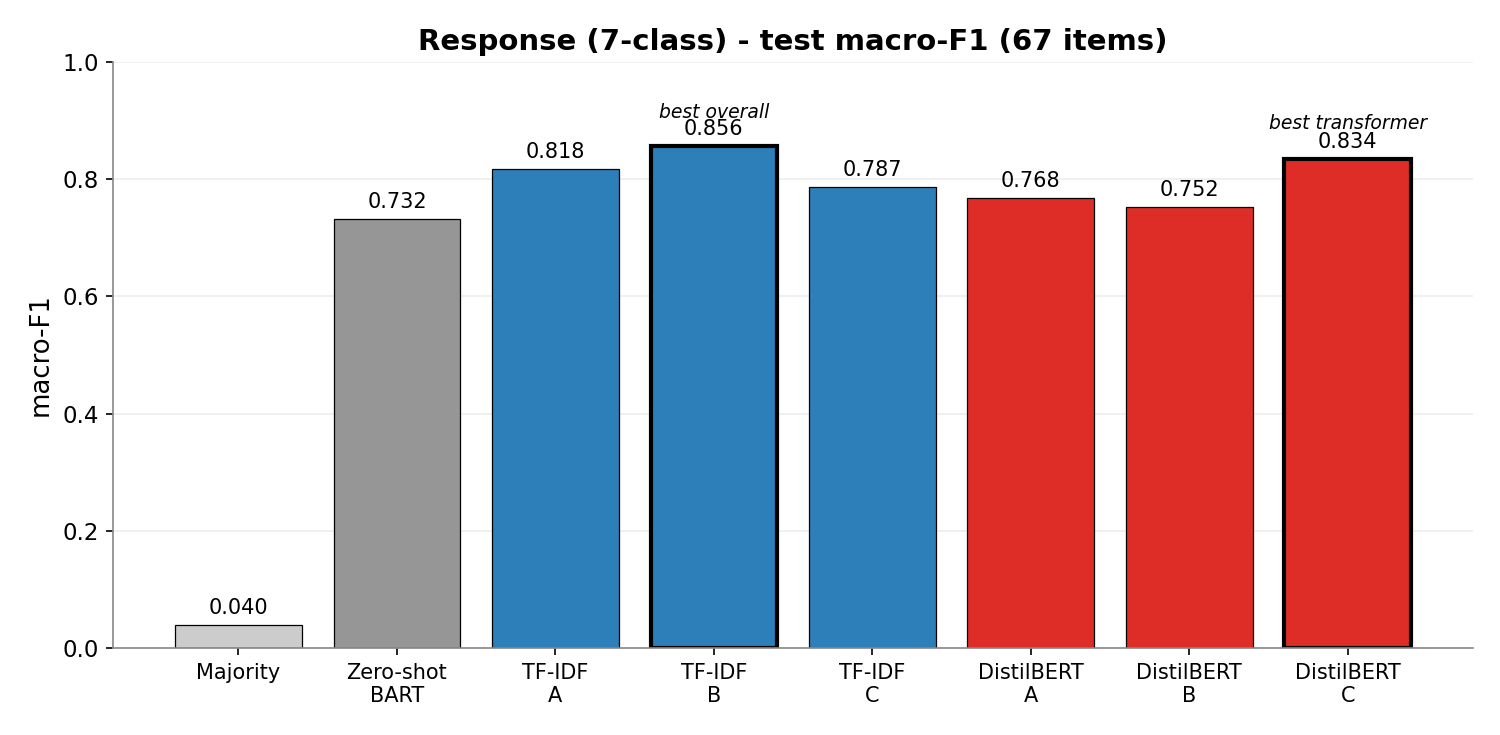
\includegraphics[width=0.95\linewidth]{results_response_macroF1.png}
  \caption{Response classification: test macro-F1 for all systems (67 items). Bold outlines mark the
  best lexical system (TF-IDF-B) and the best transformer (DistilBERT-C).}
  \label{fig:resp}
\end{figure}

\subsection{Distress classification}
Figure~\ref{fig:dist} reports macro-F1 for all distress systems. DistilBERT on tier B achieves the
highest mean (macro-F1 \textbf{0.864}, linear weighted $\kappa$ 0.851, MAE 0.113). The best lexical
model is TF-IDF nominal on tier B (0.805); the ordinal TF-IDF variant is consistently \emph{weaker}
than the nominal one (e.g.\ 0.786 vs.\ 0.805 on tier B), an honest negative result that may reflect
threshold tuning on only 45 validation items or limitations of the two-threshold decomposition.
Zero-shot BART substantially underperforms at 0.468 and is the only system with non-trivial severe errors;
the majority floor is 0.211.

\begin{figure}[t]
  \centering
  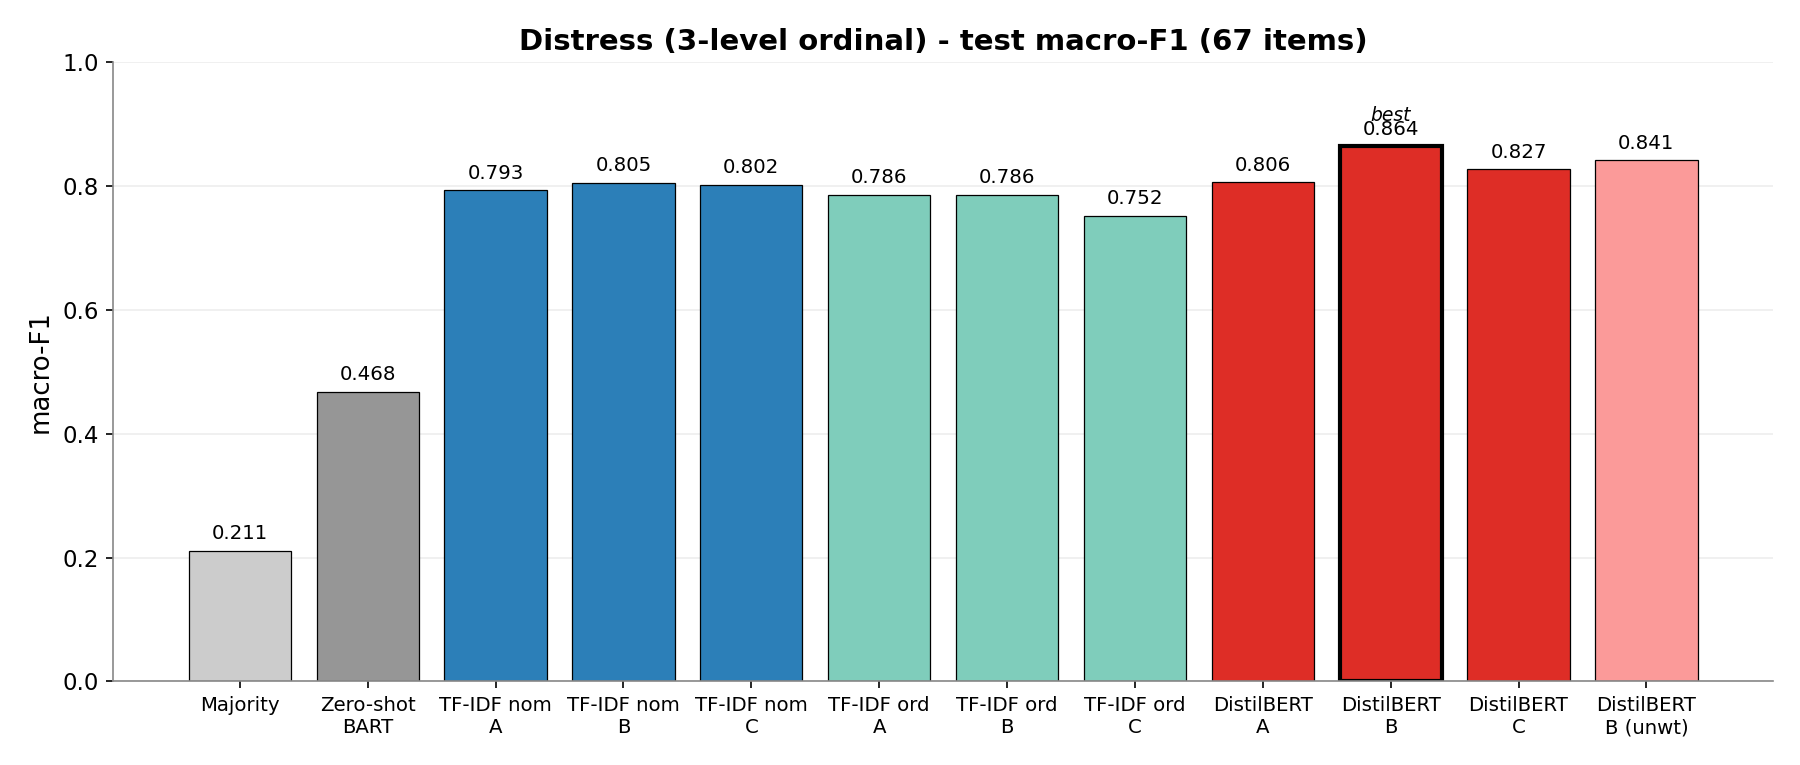
\includegraphics[width=0.97\linewidth]{results_distress_macroF1.png}
  \caption{Distress classification: test macro-F1 for all systems (67 items), including nominal and
  ordinal TF-IDF variants and an unweighted DistilBERT-B control. The bold outline marks the best
  system (DistilBERT-B).}
  \label{fig:dist}
\end{figure}

\subsection{Effect of the data tier}
Figure~\ref{fig:tier} contrasts macro-F1 across the three tiers for both model families. The peak tier
depends on both the task and the model: for response, DistilBERT achieved its highest mean on tier C
(0.768/0.752/0.834 for A/B/C), although the C-versus-A difference was not statistically resolved, while
TF-IDF peaks at B (0.818/0.856/0.787); for distress, both families
peak at B (DistilBERT 0.806/0.864/0.827; TF-IDF nominal 0.793/0.805/0.802), and the additional
consensus data in C slightly hurts. In short, \emph{more synthetic data is not uniformly better}: the
lower-purity consensus tier was associated with a higher mean in one configuration, but transferred
annotation-policy artifacts or imbalance in others.

\begin{figure}[t]
  \centering
  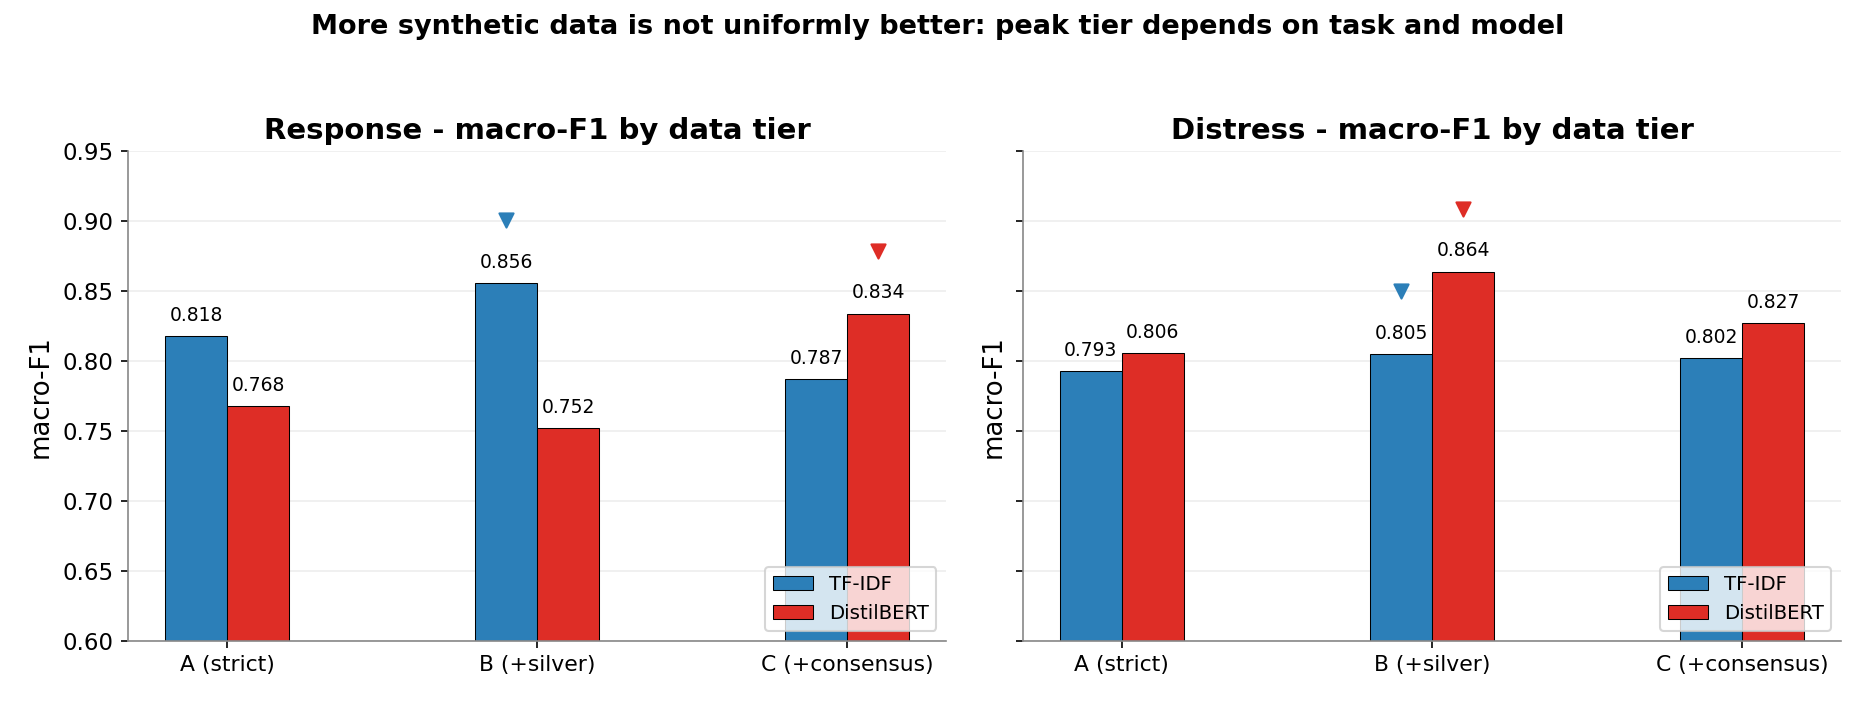
\includegraphics[width=0.97\linewidth]{results_tier_contrast.png}
  \caption{Macro-F1 by data tier (A: strict, B: $+$silver, C: $+$consensus) for both model families.
  The peak tier (marked) differs across tasks and models.}
  \label{fig:tier}
\end{figure}

\subsection{Class-weighting control}
To isolate the contribution of class weighting on the best distress configuration, we retrain
DistilBERT-B with and without class weights under identical splits, seeds, and hyperparameters
(Table~\ref{tab:weight}). Weighting yields a modest but consistent gain (macro-F1 $+0.023$, weighted
$\kappa$ $+0.023$, MAE $-0.015$), concentrated on the harder low level, with no change to the
zero-severe-error profile.

\begin{table}[t]
  \centering
  \small
  \caption{Class-weighting control on distress DistilBERT-B (identical split, seeds, hyperparameters).}
  \label{tab:weight}
  \begin{tabular}{@{}lccc@{}}
    \toprule
    Metric & Weighted-B & Unweighted-B & $\Delta$\\
    \midrule
    macro-F1 & \textbf{0.864} & 0.841 & $+0.023$\\
    weighted $\kappa$ (linear) & \textbf{0.851} & 0.828 & $+0.023$\\
    MAE (ordinal) & \textbf{0.113} & 0.128 & $-0.015$\\
    severe (low$\leftrightarrow$high) & 0.000 & 0.000 & ---\\
    \bottomrule
  \end{tabular}
\end{table}

\subsection{Statistical significance}
\label{sec:boot}
Figure~\ref{fig:boot} shows per-system 95\% bootstrap CIs for distress. DistilBERT-B
(0.853, [0.758, 0.941]) and TF-IDF nominal-B (0.805, [0.709, 0.899]) overlap substantially, and their
paired difference CI includes zero ($[-0.066, +0.164]$): the transformer's mean advantage is
\emph{not} resolved on 67 items. Both supervised systems, however, separate cleanly from zero-shot
(0.464, [0.336, 0.592]); for example, DistilBERT-B vs.\ zero-shot is $+0.391$ ([$+0.228$, $+0.555$]).
For response, the only reliably separable pair is TF-IDF-B vs.\ zero-shot ($+0.123$, [$+0.008$,
$+0.241$]); lexical and transformer systems are not separable. Supervised systems achieved higher
point estimates than zero-shot in both tasks. Bootstrap-confirmed superiority was observed for
TF-IDF-B in response and for both TF-IDF-B and DistilBERT-B in distress. The lexical-versus-transformer
comparison remained underpowered at this test-set size.

\begin{figure}[t]
  \centering
  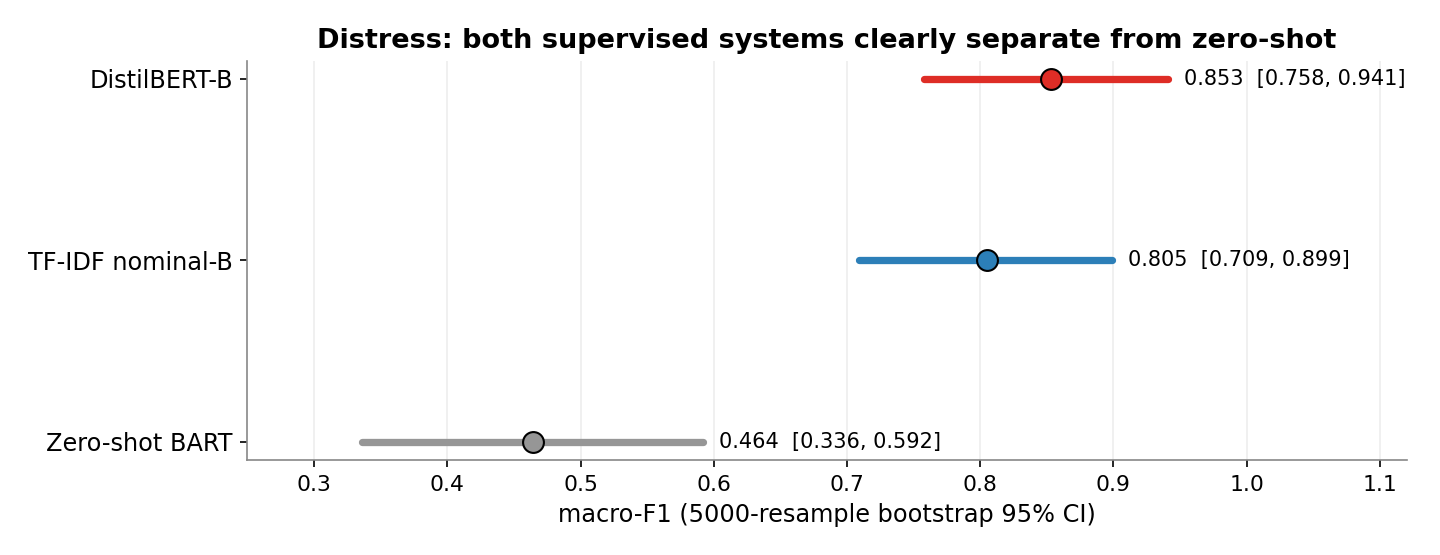
\includegraphics[width=0.92\linewidth]{results_distress_bootstrap.png}
  \caption{Distress: per-system macro-F1 with 95\% bootstrap CIs (5000 resamples). Both supervised
  systems separate from zero-shot; the two supervised systems do not separate from each other. The
  DistilBERT-B estimate uses the five-seed majority vote.}
  \label{fig:boot}
\end{figure}

\subsection{Human validation}
\label{sec:human}
\enlargethispage{\baselineskip}
A single blind annotator re-labeled the 67-item test set. Agreement with the synthetic labels was high:
for response, exact agreement was 86.6\% (Cohen's $\kappa = 0.84$); for distress, exact agreement was
83.6\% (weighted $\kappa = 0.80$ linear, $0.86$ quadratic). Comparing the best model to the human
reference on distress gives macro-F1 0.707 and weighted $\kappa$ 0.661. Crucially, agreement was strong
on human-unambiguous items and much weaker on human-ambiguous items (weighted $\kappa$ 0.817 vs.\ 0.365),
with the disagreement dominated by a systematic human-low $\rightarrow$ model-medium shift
(Figure~\ref{fig:conf}). High distress is recognized very reliably, and there are essentially no severe
(low$\leftrightarrow$high) errors. The distinction between low and medium distress is thus the least
reliable part of the label scheme and remained sensitive to subjective interpretation.

\begin{figure}[H]
  \centering
  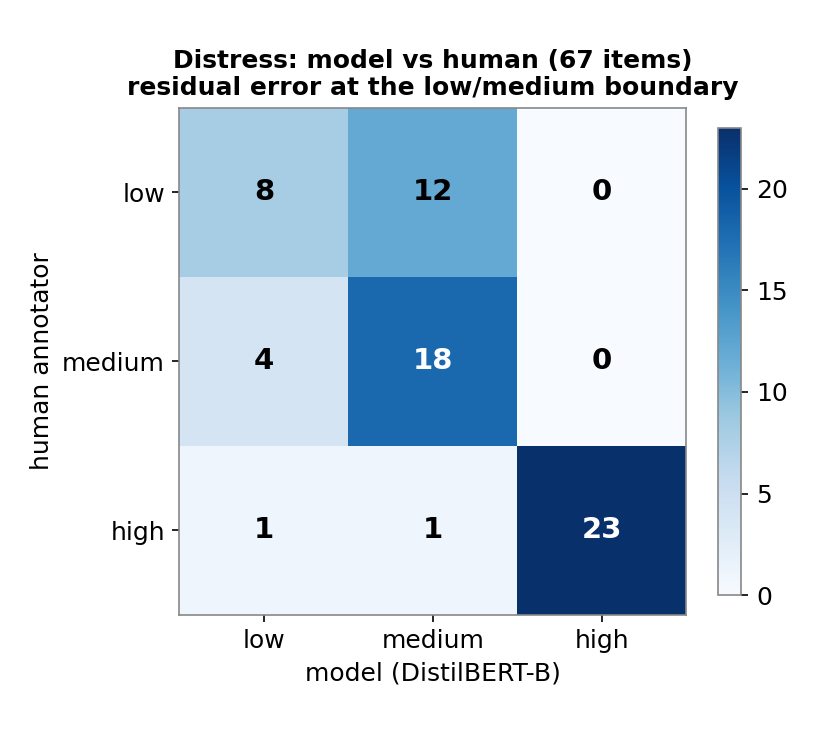
\includegraphics[width=0.5\linewidth]{results_distress_human_confusion.png}
  \caption{Distress: confusion between the best model (DistilBERT-B) and the blind human annotator on
  the 67-item test set. The residual error is concentrated at the low/medium boundary.}
  \label{fig:conf}
\end{figure}

\section{Error Analysis}
Three recurring patterns emerged. (i) \textbf{Response --- anger artifact}: anger has high agreement
with the strict synthetic label but low agreement with the independent human reading; the model
appears more closely aligned with the dual-judge annotation policy than with the independent
annotator's reading (in oncology text, anger is
often expressed as grief or protest that a human reads as sadness). (ii) \textbf{Response --- anxiety
over-prediction}: training on the consensus tier (C) inflates the predicted/support ratio for anxiety;
the cause is data composition, not the class weights. (iii) \textbf{Distress --- low/medium boundary}:
the dominant disagreement, both against the human and across models, is the systematic
human-low $\rightarrow$ model-medium shift noted above. Across the trained systems, severe errors are
nearly absent and high distress is detected well, so the residual difficulty is semantic ambiguity at
an adjacent boundary rather than an extreme ordinal error.

\section{Discussion}
The two tasks responded differently to model family and synthetic-data tier. Response labels were
highly accessible to a sparse lexical classifier, which matched the fine-tuned transformer; distress
showed a larger descriptive advantage for the transformer and a much larger gap between supervised and
zero-shot systems. This suggests distress benefits more from contextual fine-tuning than response
classification does --- yet the lexical model still reached 0.805 on distress, so this is a descriptive
advantage, not evidence that distress \emph{requires} a transformer. Practically, a TF-IDF model is a
strong, cheap, and interpretable baseline that should not be skipped, and reporting bootstrap CIs is
essential: several mean differences that look decisive are not statistically resolved at a realistic
test-set size.

\section{Limitations}
Several limitations bound our claims. The corpus is synthetic, so its class distributions reflect the
generation pipeline rather than real-world prevalence, and findings should be confirmed on real text.
The human-reference evaluation used a single annotator and therefore measures agreement with one
independent reading rather than with a multi-annotator gold standard. The test set has 67 items, which
limits the power to separate close systems (as the bootstrap makes explicit). Finally, the low/medium
distress distinction is inherently subjective and was the least reliable part of the label scheme. The
resulting classifiers are research prototypes evaluated on synthetic text and are not validated for
clinical triage or individual-level decision-making.

\section{Conclusion}
We defined a novel two-label oncology task and built a fully synthetic, attribute-controlled,
label-leakage-controlled corpus for it, audited by two independent LLM judges into quality tiers. Across
three model families, task-specific synthetic supervision was consistently useful, but its value
depended on both the task and the model family: a sparse lexical model was highly competitive for
response, while distress showed a larger (though not statistically resolved) advantage for contextual
fine-tuning. Increasing the amount of consensus-labeled data did not uniformly improve performance.
Human validation showed that the largest residual errors were concentrated at a semantically ambiguous
boundary (low/medium distress) rather than at severe failures. Future work includes a multi-annotator
gold standard, a more context-aware distress model, and validation on real (non-synthetic) text.

\begin{thebibliography}{9}
\small
\bibitem[Aperstein et al.(2025)]{apartsin2025str} Y.~Aperstein, A.~Gottlib, G.~Benita, and A.~Apartsin.
\newblock Explainable Semantic Text Relations: A Question-Answering Framework for Comparing Document
Content.
\newblock \emph{Information}, 16(12):1090, 2025.

\bibitem[Lewis et al.(2020)]{lewis2020} M.~Lewis, Y.~Liu, N.~Goyal, et al.
\newblock BART: Denoising Sequence-to-Sequence Pre-training for Natural Language Generation,
Translation, and Comprehension.
\newblock \emph{ACL}, 2020.

\bibitem[Li et al.(2023)]{li2023} Z.~Li, H.~Zhu, Z.~Lu, and M.~Yin.
\newblock Synthetic Data Generation with Large Language Models for Text Classification: Potential and
Limitations.
\newblock \emph{EMNLP}, 2023, pp.\ 10443--10461.

\bibitem[Mama et al.(2025)]{mama2025} E.~Mama, L.~Sheri, Y.~Aperstein, and A.~Apartsin.
\newblock From Fuzzy Speech to Medical Insight: Benchmarking LLMs on Noisy Patient Narratives.
\newblock \emph{arXiv:2509.11803}, 2025.

\bibitem[Sanh et al.(2019)]{sanh2019} V.~Sanh, L.~Debut, J.~Chaumond, and T.~Wolf.
\newblock DistilBERT, a distilled version of BERT: smaller, faster, cheaper and lighter.
\newblock \emph{arXiv:1910.01108}, 2019.

\bibitem[Werthaim et al.(2026)]{werthaim2026} M.~Werthaim, M.~Kimhi, A.~Apartsin, and Y.~Aperstein.
\newblock A Benchmark for Evaluating Diagnostic Questioning Efficiency of LLMs in Patient Conversations.
\newblock \emph{Scientific Reports}, 2026.

\bibitem[Xu et al.(2026)]{xu2026} S.~Xu, Z.~Wang, H.~Wang, Z.~Ding, Y.~Zou, and Y.~Cao.
\newblock LLM-based annotation and token-augmented modeling for emotional tone classification in online
cancer peer-support posts.
\newblock \emph{PLOS Digital Health}, 5(5):e0001235, 2026.

\bibitem[Yu et al.(2023)]{yu2023} Y.~Yu, Y.~Zhuang, J.~Zhang, Y.~Meng, A.~Ratner, R.~Krishna, J.~Shen,
and C.~Zhang.
\newblock Large Language Model as Attributed Training Data Generator: A Tale of Diversity and Bias.
\newblock \emph{NeurIPS Datasets and Benchmarks}, 2023.

\bibitem[Zhang et al.(2022)]{zhang2022} T.~Zhang, A.~M.~Schoene, S.~Ji, and S.~Ananiadou.
\newblock Natural Language Processing Applied to Mental Illness Detection: A Narrative Review.
\newblock \emph{npj Digital Medicine}, 2022.

\bibitem[Zheng et al.(2023)]{zheng2023} L.~Zheng, W.-L.~Chiang, Y.~Sheng, et al.
\newblock Judging LLM-as-a-Judge with MT-Bench and Chatbot Arena.
\newblock \emph{NeurIPS}, 2023.
\end{thebibliography}

\end{document}
